% Options for packages loaded elsewhere
\PassOptionsToPackage{unicode}{hyperref}
\PassOptionsToPackage{hyphens}{url}
%
\documentclass[
  english,
  man,floatsintext]{apa6}
\usepackage{lmodern}
\usepackage{amssymb,amsmath}
\usepackage{ifxetex,ifluatex}
\ifnum 0\ifxetex 1\fi\ifluatex 1\fi=0 % if pdftex
  \usepackage[T1]{fontenc}
  \usepackage[utf8]{inputenc}
  \usepackage{textcomp} % provide euro and other symbols
\else % if luatex or xetex
  \usepackage{unicode-math}
  \defaultfontfeatures{Scale=MatchLowercase}
  \defaultfontfeatures[\rmfamily]{Ligatures=TeX,Scale=1}
\fi
% Use upquote if available, for straight quotes in verbatim environments
\IfFileExists{upquote.sty}{\usepackage{upquote}}{}
\IfFileExists{microtype.sty}{% use microtype if available
  \usepackage[]{microtype}
  \UseMicrotypeSet[protrusion]{basicmath} % disable protrusion for tt fonts
}{}
\makeatletter
\@ifundefined{KOMAClassName}{% if non-KOMA class
  \IfFileExists{parskip.sty}{%
    \usepackage{parskip}
  }{% else
    \setlength{\parindent}{0pt}
    \setlength{\parskip}{6pt plus 2pt minus 1pt}}
}{% if KOMA class
  \KOMAoptions{parskip=half}}
\makeatother
\usepackage{xcolor}
\IfFileExists{xurl.sty}{\usepackage{xurl}}{} % add URL line breaks if available
\IfFileExists{bookmark.sty}{\usepackage{bookmark}}{\usepackage{hyperref}}
\hypersetup{
  pdftitle={Analysing the effect of sibling number on input and output in the first 18 months},
  pdfauthor={Catherine Laing1 \& Elika Bergelson2},
  pdflang={en-EN},
  pdfkeywords={Siblings, Lexical Development, Input Effects, Language Acquisition},
  hidelinks,
  pdfcreator={LaTeX via pandoc}}
\urlstyle{same} % disable monospaced font for URLs
\usepackage{graphicx,grffile}
\makeatletter
\def\maxwidth{\ifdim\Gin@nat@width>\linewidth\linewidth\else\Gin@nat@width\fi}
\def\maxheight{\ifdim\Gin@nat@height>\textheight\textheight\else\Gin@nat@height\fi}
\makeatother
% Scale images if necessary, so that they will not overflow the page
% margins by default, and it is still possible to overwrite the defaults
% using explicit options in \includegraphics[width, height, ...]{}
\setkeys{Gin}{width=\maxwidth,height=\maxheight,keepaspectratio}
% Set default figure placement to htbp
\makeatletter
\def\fps@figure{htbp}
\makeatother
\setlength{\emergencystretch}{3em} % prevent overfull lines
\providecommand{\tightlist}{%
  \setlength{\itemsep}{0pt}\setlength{\parskip}{0pt}}
\setcounter{secnumdepth}{-\maxdimen} % remove section numbering
% Make \paragraph and \subparagraph free-standing
\ifx\paragraph\undefined\else
  \let\oldparagraph\paragraph
  \renewcommand{\paragraph}[1]{\oldparagraph{#1}\mbox{}}
\fi
\ifx\subparagraph\undefined\else
  \let\oldsubparagraph\subparagraph
  \renewcommand{\subparagraph}[1]{\oldsubparagraph{#1}\mbox{}}
\fi
% Manuscript styling
\usepackage{upgreek}
\captionsetup{font=singlespacing,justification=justified}

% Table formatting
\usepackage{longtable}
\usepackage{lscape}
% \usepackage[counterclockwise]{rotating}   % Landscape page setup for large tables
\usepackage{multirow}		% Table styling
\usepackage{tabularx}		% Control Column width
\usepackage[flushleft]{threeparttable}	% Allows for three part tables with a specified notes section
\usepackage{threeparttablex}            % Lets threeparttable work with longtable

% Create new environments so endfloat can handle them
% \newenvironment{ltable}
%   {\begin{landscape}\centering\begin{threeparttable}}
%   {\end{threeparttable}\end{landscape}}
\newenvironment{lltable}{\begin{landscape}\centering\begin{ThreePartTable}}{\end{ThreePartTable}\end{landscape}}

% Enables adjusting longtable caption width to table width
% Solution found at http://golatex.de/longtable-mit-caption-so-breit-wie-die-tabelle-t15767.html
\makeatletter
\newcommand\LastLTentrywidth{1em}
\newlength\longtablewidth
\setlength{\longtablewidth}{1in}
\newcommand{\getlongtablewidth}{\begingroup \ifcsname LT@\roman{LT@tables}\endcsname \global\longtablewidth=0pt \renewcommand{\LT@entry}[2]{\global\advance\longtablewidth by ##2\relax\gdef\LastLTentrywidth{##2}}\@nameuse{LT@\roman{LT@tables}} \fi \endgroup}

% \setlength{\parindent}{0.5in}
% \setlength{\parskip}{0pt plus 0pt minus 0pt}

% \usepackage{etoolbox}
\makeatletter
\patchcmd{\HyOrg@maketitle}
  {\section{\normalfont\normalsize\abstractname}}
  {\section*{\normalfont\normalsize\abstractname}}
  {}{\typeout{Failed to patch abstract.}}
\patchcmd{\HyOrg@maketitle}
  {\section{\protect\normalfont{\@title}}}
  {\section*{\protect\normalfont{\@title}}}
  {}{\typeout{Failed to patch title.}}
\makeatother
\shorttitle{Effect of sibling number on language}
\keywords{Siblings, Lexical Development, Input Effects, Language Acquisition\newline\indent Word count: X}
\DeclareDelayedFloatFlavor{ThreePartTable}{table}
\DeclareDelayedFloatFlavor{lltable}{table}
\DeclareDelayedFloatFlavor*{longtable}{table}
\makeatletter
\renewcommand{\efloat@iwrite}[1]{\immediate\expandafter\protected@write\csname efloat@post#1\endcsname{}}
\makeatother
\usepackage{lineno}

\linenumbers
\usepackage{csquotes}
\ifxetex
  % Load polyglossia as late as possible: uses bidi with RTL langages (e.g. Hebrew, Arabic)
  \usepackage{polyglossia}
  \setmainlanguage[]{english}
\else
  \usepackage[shorthands=off,main=english]{babel}
\fi

\title{Analysing the effect of sibling number on input and output in the first 18 months}
\author{Catherine Laing\textsuperscript{1} \& Elika Bergelson\textsuperscript{2}}
\date{}


\affiliation{\vspace{0.5cm}\textsuperscript{1} University of York, York, UK\\\textsuperscript{2} Duke University, Durham, NC, USA}

\abstract{
The `sibling effect' has been widely reported in studies examining a breadth of topics in the academic literature, suggesting firstborn children are advantaged across a range of cognitive, educational and health-based measures compared with their later-born peers. Expanding on this literature using naturalistic home-recorded data and parental vocabulary report, we find that early language outcomes vary by number of siblings. Specifically, we find that children with two or more older siblings - but not one - had smaller vocabularies at 18 months, and heard less input from caregivers across several measures. We discuss implications regarding what infants experience and learn across a range of family sizes in infancy.
}



\begin{document}
\maketitle

The \enquote{sibling effect} - that is, the apparent advantage for earlier-born versus later-born children - was noted as far back as the 1800s, when Galton (1874) observed that notable \enquote{English men of science} were often firstborns. Galton (1874, p. 35) posited that these men \enquote{would generally have more attention in {[}their{]} infancy\ldots than {[}their{]} younger brothers and sisters}, thereby giving them more of a chance of later success. Current research finds some evidence to support these claims, showing that those who have fewer older siblings are more likely to do better than their laterborn siblings in a range of domains, including educational outcomes (Esposito, Kumar, \& Villaseñor, 2020; Monfardini \& See, 2016), overall earnings (Behrman \& Taubman, 1986; Kantarevic \& Mechoulan, 2006), and some aspects of physical and mental health (Black, Devereux, \& Salvanes, 2016). This work suggests that there may be marked economic, social and physical advantages for children with fewer older siblings.

In this paper, we consider the role of siblings in the early language environment. Prior work finds that educational attainment is shaped by early language outcomes (Anderson \& Freebody, 1981; Marchman \& Fernald, 2008); e.g., one study finds that children with higher vocabulary scores at age 2 did better on a range of language and literacy measures at age 10-11 (Lee, 2011). Given that quality and quantity of the early linguistic input can predict lexical advance (Cartmill et al., 2013; Ferjan Ramírez, Lytle, \& Kuhl, 2020), it may be the case that having more siblings in the early learning environment has a negative effect on language development. With this in mind, we use naturalistic home-recorded data to measure input in earlier- and later-born infants in relation to their lexical development over the first 18 months of life.

Many studies assume an optimum environment for early language development, whereby the input is tailored to the infant's needs, changing over time as language capacity develops (e.g.~Soderstrom, 2007; Stern, Spieker, Barnett, \& MacKain, 1983). However, for many infants and for many reasons, language acquisition does not take place in such a setting; various domestic and social factors are known to affect the learning environment, including the presence of older siblings in the home (Fenson et al., 1994). According to the United States Census Bureau (2010), around one third of children are born into households with at least one other infant present, and one in every five infants is acquiring language in a household shared with two or more other children. Similar statistics are reported for British infants (Office for National Statistics, 2018), where the average household has 1.75 children, and 15\% of households have three children or more.

Consistent with the broader literature in this area, language development research has shown that infants born to households with older children may experience disruption to their linguistic trajectory. Fenson and colleagues (1994) found that by 30 months of age, children with older siblings performed worse than those with no siblings across measures of productive vocabulary, word combinations, and mean length of utterance (MLU). This disadvantage may be manifested in input differences between first- and later-born children: infants with older siblings hear less speech aimed specifically at them, and what they do hear is understood to be linguistically less supportive of early language development (Hoff-Ginsberg, 1998; Oshima-Takane \& Robbins, 2003). The sex of the older siblings may also have an effect on a child's development: Havron and colleagues (2019) expand on this to show that the effect is manifested largely in the presence of an older brother - children with an older sister did not differ in their language skills from those with no siblings, whereas children with an older brother had significantly lower language skills. Furthermore, some studies have noted linguistic \textbf{advantages} for later-borns (Oshima-Takane, Goodz, \& Derevensky, 1996). In particular, they may have an advantage in the development of social-communicative skills (Hoff, 2006) and some aspects of syntactic development (Oshima-Takane et al., 1996), as well as being more able to join in with conversations (Dunn \& Shatz, 1989).

Numerous studies have attempted to better understand the mechanisms behind this issue, with comparisons of language acquisition across first- and later-borns, and analyses of mothers' input in dyadic (infant + mother) and triadic (infant + mother + older sibling) situations. Findings tend to be mixed, but overall two general conclusions can be drawn. First, analyses consistently show that there is a disadvantage in early language acquisition for infants with older siblings (Berglund, Eriksson, \& Westerlund, 2005; Fenson et al., 1994; Pine, 1995; Zambrana, Ystrom, \& Pons, 2012). However, the difference is often reported as being only marginal, and only typical of the earliest stages of language learning. Fenson and colleagues (1994) highlight a weak but significant negative correlation between birth order and word production over time: infants with more siblings acquired fewer words over the course of their analysis (up until age 2;6). In an analysis of 18 infants, Pine (1995) reports an advantage in lexical acquisition for first-born infants in early development, as infants with siblings were slower to reach the 50-word point. However, by the 100-word point this difference had dissipated, suggesting that later-born infants soon catch up with their first-born peers. This is consistent in studies observing the development of social and interactive understanding: Hoff-Ginsberg (1998) shows first-borns to have better lexical and syntactic skills up until 2;5, but later-born infants had better conversational abilities during the same time-period. Adding to this picture, Oshima-Takane and colleagues (1996) show that second-born infants use significantly more pronouns in their speech at age 1;9, suggesting that there may be at least some advantage for the development of syntax and lexical categories amongst later-born infants.

The second finding to appear consistently in the literature pertains to differences in input quality during dyadic and triadic interactions. Findings show that infants with no siblings receive not only more input overall, but also higher-quality input. A range of different input quality measures have been adopted in the literature, including speech rate (number of utterances in relation to utterance duration), richness of vocabulary (number of word roots produced in a session), MLU, responses to children's utterances, and type-token ratio, among others (Hoff-Ginsberg, 1991, 1998; Oshima-Takane \& Robbins, 2003; Stafford, 1987). These measures are believed to reflect an input that is supportive of early language development, and across studies it is generally observed that infants with siblings are presented with lower input quality (across various operationalizations) than those without siblings; e.g., second-born infants receive less supportive maternal input even in dyadic interactions (Hoff-Ginsberg, 1998). And of course, the presence of siblings means that infants will also hear speech from older children. However, input from sibilngs versus parents is likely different in many ways. For instance, in a study comparing input quality in mother-infant versus sibling-infant dyads, Hoff-Ginsberg and Krueger (1991) show mothers' input to be more linguistically supportive than input from older siblings. While this study found more supportive input from older (7-8 yo) vs.~younger (4-5 yo) siblings, this input was still lower quality than that of the mother (though cf.~Havron and colleague's recent work that the size of the age-gap may not have repercussions on the target child's language skills ({\textbf{???}}).

Indeed, the very presence of a sibling in the linguistic environment changes the way language is used. When siblings are present in triadic interactions, mothers' input is more focused on regulating behaviour, as opposed to the language-focused speech that is common in dyadic contexts (Oshima-Takane \& Robbins, 2003). These advantages are consistent in input quantity as well, as infants with no siblings not only hear speech that is linguistically more supportive, but they also hear more input overall. Reports show that MLU is longer in the input of first-born infants (Hoff-Ginsberg, 1998; but see also Oshima-Takane \& Robbins, 2003 for a comparison of dyadic and triadic contexts) who also hear more questions directed at them than later-borns. Both Jones and Adamson (1987) and Oshima-Takane and Robbins (2003) report no difference between the number of word types produced by mothers in dyadic and triadic settings, but the proportion of speech directed at the target infant is drastically reduced when input is shared with siblings.

As Hoff (2006) explains, infants with siblings have less experience of speech directed at them, but they do have an advantage over their first-born peers in that they are subject to more overheard speech. Indeed, the input of first-borns may be explicitly tailored to their needs, but equally this means it might be less varied, and may not support the development of communication and even grammatical skills to the same extent as input shared with older siblings. In her analysis of the sibling effect on children's early language environment, Woollett (1986) highlights that focusing on the purely linguistic aspects of an infant's input does not best represent the real experience of learning language, which is after all a highly social tool, dependent on more than phonetics and syntax for its effective acquisition. She states that \enquote{taking a wider view of language may make the search for one register to facilitate language development seem a very limited goal} (1986, p.243). She goes on to posit that the features of infant-directed speech (IDS) that we understand to facilitate language learning may, in other respects, hinder the process. This is supported by findings from Oshima-Takane, Goodz and Derevensky (1996), who combine analyses of the input with experimental evidence of infants' on-line linguistic skills. The authors show that infants with siblings hear more pronouns in their input, and are consequently better able to use pronouns in their own speech; they also answered more questions about pronouns correctly when tested in an experimental task. However, Wellen (1985) points out that infants' passive observation of successful interactions between mother and sibling is much less important for language learning than actually participating in interactions. While there may be a role for overheard speech, it does not override the importance of dedicated one-to-one interactions between infant and mother. Findings from Ramírez-Esparza and colleagues (2014) support this by showing that infants' later language development is shaped by the amount of one-to-one interactions with a caregiver. However, Barton and Tomasello (1991) show that by as early as 19 months, infants with siblings are already able to take part in triadic conversations, supporting an advantage for the presence of other children in the learning environment. Triadic conversations were almost three times longer than dyadic conversations, and the authors suggest that this may have an important effect on the learning dynamic of the situation: infants are under less pressure to participate in a triadic interaction, meaning the conversation can continue even when the infant is unable to respond. As a result, the infants took more conversational turns in triadic interactions than dyadic ones.

Taken together, it seems that there is an early disadvantage in lexical development for laterborn children, which may be redressed when it comes to syntactic and communicative development. However, given that vocabulary size is a known key predictor of later educational success (Lee, 2011; Marchman \& Fernald, 2008), combined with studies showing that laterborns have lower educational attainment by high school (Esposito et al., 2020; Monfardini \& See, 2016), the disadvantage in early lexical development amongst laterborns may be particularly important.

In analyzing infants' lexical development in relation to the presence of older siblings in their household, the present work expands on the extant literature in two key ways. First, while prior work generally considered birth order as a binomial factor (i.e.~comparing first-born infants with second-borns (e.g.~Oshima-Takane \& Robbins, 2003), or \enquote{later-borns} (e.g.~Hoff-Ginsberg, 1998), potentially missing graded effects, we consider how \emph{discrete sibling number} (i.e.~how many siblings a child has) is linked to an infants' lexical development and the quality of their input. Second, much of the existing literature in this area is drawn from questionnaire data or brief interactions recorded in the lab (but see Dunn \& Shatz, 1989 for a study of naturalistic home-recorded data), rather than naturalistic day-to-day interaction sin the home. In contrast, we use an existing corpus of daylong audio-recordings in concert with vocabulary checklists for our analysis. Based on the prior work summarized above, our overall prediction was that both the language environment and infants early vocabulary would vary as a function of how many older siblings they have.

\hypertarget{hypotheses}{%
\section{Hypotheses}\label{hypotheses}}

Research has already shown that early lexical development is more advanced among first-born infants (e.g.~Hoff-Ginsberg, 1998). We expect to see the same effect in our data, but we hypothesize that the closer granularity of this analysis will show a gradient decline in infants' lexical abilities in relation to an increasing number of siblings.
With regard to the infants' linguistic environment, we hypothesize that increased sibling number will have a negative effect on factors of the early input that are known to support language development. To test this, we adopt three input measures, as established in the literature as being important for early language learning:

\begin{enumerate}
\def\labelenumi{\arabic{enumi})}
\item
  \textbf{Amount of input} will decline as sibling number increases. Mothers' attention will be divided across a larger group of children, and as a result the proportion of input from the mother will be lower for infants with more siblings. In addition, these infants will experience more input from other children in the home. Amount of overall input is an important predictor of language development in the longer term (Huttenlocher, Haight, Bryk, Seltzer, \& Lyons, 1991), as is amount of one-to-one input from the caregiver (Ramírez-Esparza et al., 2014). We thus expect this to be an important determiner of infants' lexical production skills at 18 months.
\item
  \textbf{More \enquote{learnable} words} (words that tend to be acquired earlier, Fenson et al., 1994) will occur in the input of infants with fewer siblings, and this will decrease as sibling number increases. Input from older children will generate a wider variety of lexical items in the input, including words directed to and produced by siblings, some of whom will still be young language learners themselves. As a result, in homes with older siblings, we predict fewer input words will be oriented specifically towards the infant.
\item
  \textbf{Amount of object presence} (the presence of the object being referred to in the input, e.g.~mother says \enquote{cat} when there is a cat in the room) will decrease as sibling number increases. As caregivers' attention is drawn away from one-to-one interactions with the infant, there will be less opportunity for contingent talk. Moreover, less learnable words are also expected to be less imageable, and thus less likely to be presented alongside caregivers' utterances. The co-occurrence of words alongside their associated objects is thought to contribute to the earlier learning of nouns over verbs (Bergelson \& Swingley, 2013). Furthermore, object presence is more suited to instances of joint visual attention with the caregiver, again supporting the word learning process through the concrete mapping of word to referent (Gleitman, Cassidy, Nappa, Papafragou, \& Trueswell, 2005).
\end{enumerate}

\hypertarget{methods}{%
\section{Methods}\label{methods}}

We analyze data from the SEEDLingS corpus (Bergelson, Amatuni, Dailey, Koorathota, \& Tor, 2019), a longitudinal set of data incorporating home recordings, parental reports and experimental studies from the ages of 0;6 to 1;6. The present study draws on the parental report data, and annotations of hour-long home video recordings, taken on a monthly basis during data collection.

\hypertarget{participants}{%
\subsection{Participants}\label{participants}}

Forty-four families in New York State completed the year-long study. Infants (21 females) were from largely middle-class households; 33 mothers had attained a B.A. degree or higher. All infants had normal birthweight with no reported speech or hearing problems. Forty-two infants were Caucasian; two were from multi-racial backgrounds.

\hypertarget{materials}{%
\subsection{Materials}\label{materials}}

\textbf{Parental report data} The present analyses draw on data from vocabulary checklists (Macarthur-Bates Communicative Development Inventory, hereafter CDI; Fenson et al., 1994), administered monthly from 0;6 to 1;6, along with a demographics questionnaire. Because the majority of infants did not produce their first word until around 0;11 according to CDI reports (M=10.70, SD=2.22)\footnote{Note that reported word production began earlier than observed word production (i.e.~in the video recordings) but this difference was not statistically significant (see Moore, Dailey, Garrison, Amatuni, \& Bergelson, 2019).}, we use CDI data from 0;10 onwards in our analysis. CDI production data for each month is taken as a measure of the infants' lexical development over the course of the analysis period.

\textbf{Home video data} Every month between 0;6 and 1;5, infants were recorded for one hour in their home, capturing a naturalistic representation of each infant's day-to-day input. Infants wore a hat with two small Looxcie video cameras attached, one pointed slightly up, and one pointed slightly down; this allowed us to record the scene from the infants' perspective. In the event that infants refused to wear the hats, caregivers wore the same kind of camera on a headband. Additionally, a camcorder was set up in the home. Object words (i.e.~concrete nouns) deemed to be directed to or attended by the child were annotated by trained coders. Here we examine annotations for speaker, i.e.~who produced a word, and object presence, i.e.~whether the word's referent was present and attended to by the infant.

\hypertarget{procedure}{%
\subsection{Procedure}\label{procedure}}

We analyzed number of siblings based on parental report in the demographics questionnaires completed at 0;6 (R: 0-4). Siblings were on average 4.05 years older than the infants in this study (Mdn days: 1477, SD: 1477, R: 0-17 years).\footnote{For six infants, siblings' exact birthdates were not provided, and so age difference was estimated by subtracting the infant's age (6 months) from the sibling's age in years, as listed on the questionnaire (e.g.~if a sibling was 5 years old, they were classed as being 4.5 years older than the infant).} All siblings lived in the household with the infant, and all were older than or of the same age as the infant in question.\footnote{Two infants in the dataset were dizygotic twins; our pattern of results holds with or without these infants.}

\hypertarget{input-measures}{%
\subsection{Input measures}\label{input-measures}}

Three input measures were derived based on the annotations of concrete nouns in this corpus, each pertaining to aspects of the input that are established as important in early language learning: \textbf{overall household input} (how many concrete nouns does each infant hear?), \textbf{early-acquired words} (how much of this input is \emph{early-learned} nouns?), and \textbf{object presence} (how much of this input is referentially transparent?). Each is described in further detail below.

\emph{Household Input} reflects how many nouns infants heard in the recordings from their mother, father and (where relevant) siblings. Other speakers' input was relatively rare during video recordings, accounting for 0.09\% of input overall (SD=0.24, and is excluded from our analysis. This measure of the early language environment is based on evidence showing strong links between the amount of speech heard in the early input and later vocabulary size (Anderson, Graham, Prime, Jenkins, \& Madigan, 2021). This analysis considers only nouns produced by speakers in the child's environment, as concrete nouns are acquired earlier in development in English and cross-linguistically (Braginsky, Yurovsky, Marchman, \& Frank, 2019). Note that Bulgarelli and Bergelson (2020) found that, for the same corpus of data, noun production correlated strongly with automated adult word count estimates; we can thus assume that higher noun count in this data indicates higher input across the board.

\emph{Early-acquired words} reflects the proportion of object word lemmas in the parental input that appeared on the \enquote{Words \& Gestures} communicative development inventory (CDI, Fenson et al., 1994). This CDI form offers an inventory of words typically acquired by infants from the United States between the ages of 8 and 18 months (Fenson et al., 2007). The CDI items were established based on a sample of over 1,700 infants (\textasciitilde50\% firstborn, 73\% White, 44\% of mothers with a college diploma), and so the CDI is taken as a standardized proxy of words typically acquired by infants in early development. Words found on the CDI are, by definition, early-learned, though somewhat variable in their age of acquisition and in the reasons underlying their learnability. Thus, CDI words like \emph{foot} and \emph{banana} are acquired earlier than non-CDI words like \emph{jet ski} or \emph{wheel}. Frank and colleagues (2021) show that the earliest-learned words are very similar across languages, suggesting a conceptual bias towards some words over others in early acquisition (though many factors, e.g.~frequency, concreteness, phonological complexity, are relevant as well). Note also that our measure of early-acquired words in the input is the same as our measure of infant vocabulary development (i.e., the CDI wordlist), and so captures broad parallels between the words parents say and the words their infants are reported to have acquired.

\emph{Object Presence} was coded for each object word in the home recordings based on whether or not the annotator determined the object in question as present and attended to by the child. This is a metric of referential transparency, which has been suggested to aid in learning (Bergelson \& Swingley, 2013). Bergelson and Aslin (Bergelson \& Aslin, 2017) found that word-object co-presence in the home correlated with infants' ability to recognise the same words in an eye-tracking experiment, suggesting an advantage for object labeling in word learning. This is consistent with findings from Cartmill and colleagues (2013), who found that more referentially-transparent interactions with the caregiver (as judged by adult speakers observing videos where target words were blanked out) predicted larger vocabulary size at 54 months. Indeed, presence of the labelled object decreases the ambiguity of the learning environment (Yurovsky, Smith, \& Yu, 2013), and may be a crucial component of supportive contingent talk (McGillion, Pine, Herbert, \& Matthews, 2017).

In the following analyses, we consider infants' productive vocabulary alongside our three input measures: amount of household input, number of early-acquired nouns in the input, and extent of object presence in the input, as a function of sibling number. These measures index established measures of both input quality and quantity (though we make no distinction between quality/quantity of input here), and will be analysed in relation to infants' reported productive vocabulary (all word types included) as our dependent measure. Since the raw data are highly skewed, log-transformed data\footnote{1 was added to the raw infant production data of all infants before log-transformation to retain infants with vocabularies of 0.} and/or proportions are used for statistical analysis. All figures display non-transformed data for interpretive ease.

\hypertarget{results}{%
\section{Results}\label{results}}

Vocabulary development was highly variable across the 44 infants. By 18 months, 2 infants produced no words, while mean productive vocabulary was 60.28 words (SD=78.31, Mdn=30.50). One female infant had a substantially larger reported vocabulary (3SDs above the mean monthly vocabulary score) between 1;1 and 1;6 and was classed as an outlier. We removed her from our data, leaving 43 infants (20 females) in the present analysis. Infants had one sibling on average (M=0.86, Mdn=1, SD=1.09). See Table \ref{tab:table-sibling-number}.

\begin{table}[H]

\begin{center}
\begin{threeparttable}

\caption{\label{tab:table-sibling-number}Sibling number by female and male infants.}

\small{

\begin{tabular}{llll}
\toprule
n Siblings & \multicolumn{1}{c}{Female} & \multicolumn{1}{c}{Male} & \multicolumn{1}{c}{Total}\\
\midrule
0 & 9 & 12 & 21\\
1 & 7 & 6 & 13\\
2 & 2 & 3 & 5\\
3 & 2 & 0 & 2\\
4 & 0 & 2 & 2\\
Total & 20 & 23 & 43\\
\bottomrule
\end{tabular}

}

\end{threeparttable}
\end{center}

\end{table}

\hypertarget{model-structure-for-fixed-and-random-effects}{%
\subsection{Model structure for fixed and random effects}\label{model-structure-for-fixed-and-random-effects}}

All reported models were generated in R (R Core Team, 2019) using the \emph{lmerTest} package to run linear mixed-effects regression models (Kuznetsova, Brockhoff, \& Christensen, 2017). P-values were generated by likelihood ratio tests resulting from nested model comparison. All models include infant as a random effect. All post-hoc tests are two-sample, two-tailed Wilcoxon Tests, given that all but one of our variables differed significantly from normal by Shapiro tests. We thus opted to run non-parametric tests for all post-hoc comparisons. Where multiple post-hoc comparisons are run on the same dataset, Bonferroni corrections are applied with an adjusted threshold of \(a\)=0.03, accounting for two between-group comparisons (no siblings vs.~one sibling, one sibling vs.~multiple siblings; see below).

Before considering sibling status, we first modelled infants' productive vocabulary as a function of age, sex, and mother's education. There was no effect of sex on productive vocabulary at 18 months (\emph{p}=.632), and no correlation with mothers' education level (across five categories from High School to Doctorate; \emph{r} = -0.01, \emph{p}=.139). As expected, age had a significant effect on productive vocabulary (\emph{p}\textless{} .001), and so we include age as a fixed effect in all subsequent models. Because we expected that maternal age and education might have an effect on both sibling number and infant productive vocabulary, we ran further correlations to test these variables. There was no correlation between mother's education and number of siblings (\emph{r} = -0.01, \emph{p}=.928), and a marginal positive correlation between mother's age and number of siblings (Spearman's \emph{r} = 0.28, \emph{p}=.069); older mothers tended to have more children. However, no correlation was found between mothers' age and productive vocabulary at 18 months (\emph{r} = -0.04, \emph{p}=.822).

\hypertarget{effect-of-siblings-on-infants-productive-vocabulary}{%
\subsection{Effect of siblings on infants' productive vocabulary}\label{effect-of-siblings-on-infants-productive-vocabulary}}

We next modeled the effect of siblings on productive vocabulary. Starting with a binary variable (0 vs.~\textgreater0 siblings), our model revealed no effect for the presence of siblings on productive vocabulary when we included month as a fixed effect (\(\chi^2 (1)\) = 2.27, \emph{p}=.132). We then modelled aggregated groups (None vs.~One vs.~2+) and discrete sibling number (0 vs.~1 vs.~2 vs.~3 vs.~4 siblings). In both cases, models with siblings accounted for more variance in productive vocabulary than models without it (see Table \ref{tab:table-sibling-model-output}).

\begin{table}[H]

\begin{center}
\begin{threeparttable}

\caption{\label{tab:table-sibling-model-output}Output from regression models comparing language development over time in relation to sibling number (binary, grouped and discrete variables). Month was included in each model as a fixed effect; subject was included as a random effect.}

\small{

\begin{tabular}{llll}
\toprule
Model & \multicolumn{1}{c}{Df} & \multicolumn{1}{c}{Chisq} & \multicolumn{1}{c}{p value}\\
\midrule
0 vs. >0 siblings & 1.00 & 2.27 & 0.13\\
Sibling group & 2.00 & 7.96 & 0.02\\
Sibling number & 1.00 & 6.24 & 0.01\\
\bottomrule
\end{tabular}

}

\end{threeparttable}
\end{center}

\end{table}

In short, having more siblings was associated with a smaller productive vocabulary over the course of early development. This is consistent with previous findings (Hoff-Ginsberg, 1998; Pine, 1995). Moreover, for each additional sibling, infants acquired 31\% fewer words. Looking at differences between sibling groups (0 vs.~1 vs.~2+ siblings), we see that infants with one sibling produce only 5\% fewer words than firstborns over the course of our analysis, while infants with two or more siblings produce 94\% fewer words. See Table \ref{tab:table-data-summary} and Figure \ref{fig:Figure-SibGroup}. Post-hoc Wilcoxon Rank Sum tests comparing reported productive vocabulary at 18 months revealed significantly larger vocabularies for infants with one sibling compared to those with two or more siblings (\emph{W}=5, \emph{p} = .004), but no difference between infants with one sibling and those with no siblings (\emph{W}=79.50, \emph{p} = .631; Bonferroni corrections applied).

\begin{figure}
\centering
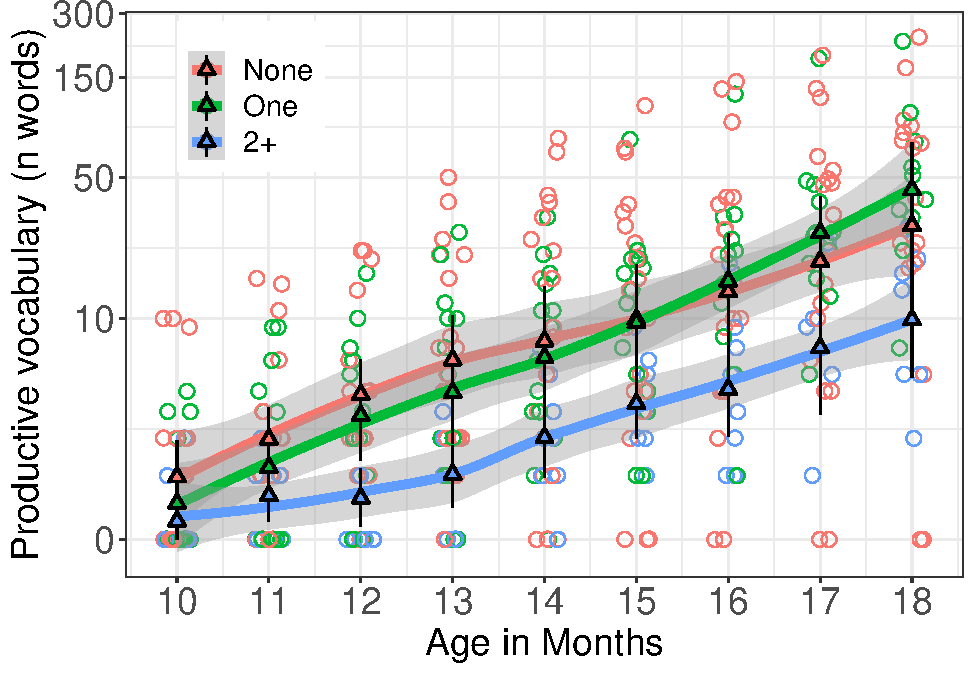
\includegraphics{SiblingsStudyText_files/figure-latex/Figure-SibGroup-1.pdf}
\caption{\label{fig:Figure-SibGroup}Productive vocabulary acquisition over time. Colors denote sibling group; line with grey confidence band reflects local estimator (loess) fit over individual infants' vocabulary at each month. Triangles indicate mean with bootstrapped CIs computed over each month's data. Points (jittered horizontally) show individual infants' vocabulary size at each month. Y-axis utilizes log-transformed vertical spacing for visual clarity.}
\end{figure}

\hypertarget{effect-of-siblings-on-infants-input}{%
\subsection{Effect of siblings on infants' input}\label{effect-of-siblings-on-infants-input}}

Having established that infants' productive vocabulary varied as a function of how many siblings they had, we turn to our three input measures to test whether input varied by a child's sibling status. To keep relatively similar Ns across groups we used the 0 vs.~1 vs.~2+ siblings division. That said, with the exception of household input (see Supplementary Data) all reported results hold if we model discrete sibling number as a fixed effect instead.

As with our previous analysis, we first modeled infants' input (maternal input only) as a function of age, sex and maternal education. This time, there was no effect for age, nor sex or maternal education (\emph{p}s all\textgreater.261) on the amount of input produced by mothers. We therefore excluded all three variables from our models.

\hypertarget{parental-input}{%
\subsubsection{Parental Input}\label{parental-input}}

\begin{table}

\caption{\label{tab:table-data-summary}Data summary of all three input variables and reported vocabulary size at 18 months.}
\centering
\begin{tabular}[t]{ccccccc}
\toprule
\multicolumn{1}{c}{ } & \multicolumn{2}{c}{No siblings} & \multicolumn{2}{c}{1 sibling} & \multicolumn{2}{c}{2+ siblings} \\
\cmidrule(l{3pt}r{3pt}){2-3} \cmidrule(l{3pt}r{3pt}){4-5} \cmidrule(l{3pt}r{3pt}){6-7}
Variable & none m & none sd & 1 m & 1 sd & 2 m & 2 sd\\
\midrule
\% early-acquired words in input & 0.85 & 0.08 & 0.84 & 0.08 & 0.79 & 0.11\\
\% object presence in input & 0.66 & 0.14 & 0.55 & 0.15 & 0.45 & 0.17\\
N Input utterances, 10-17 months & 63.96 & 112.87 & 65.35 & 92.59 & 35.71 & 50.50\\
Productive Vocabulary 18m & 58.89 & 60.76 & 92.64 & 111.42 & 13.00 & 9.49\\
\bottomrule
\end{tabular}
\end{table}

\begin{figure}
\centering
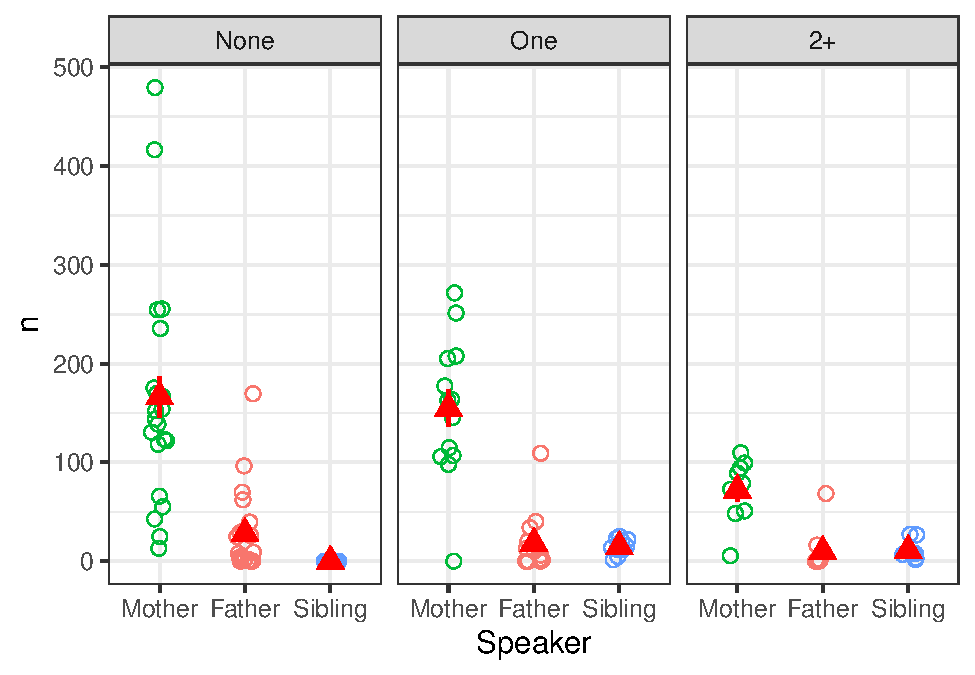
\includegraphics{SiblingsStudyText_files/figure-latex/Figure-Speaker-count-1.pdf}
\caption{\label{fig:Figure-Speaker-count}Mean number of words produced by Mothers, Fathers and Siblings across sessions recorded between 10-17 months. Circles represent values for individual infants; red triangles show group means.}
\end{figure}

Mothers provided the largest proportion of the infants' overall input across the sample (83\%, M=155.39 object words, Mdn=134.50, SD=127.02). Fathers accounted for an average of 13\% (M=23.49, Mdn=0, SD=51.58), while infants with siblings received around 5\% of their input from their brothers and sisters (M=17.29, Mdn=12, SD=19.82). See Table \ref{tab:table-data-summary} and Figure \ref{fig:Figure-Speaker-count}. We tested overall quantity of input (aggregated across mothers, fathers, and siblings) in our model, and a significant effect was found (\(\chi^2 (2)\) = 18.64, \emph{p}\textless{} .001). We then ran post-hoc tests to compare mean amount of input across sibling groups. With Bonferroni corrections applied (\(a\)=0.03), these showed a significant difference in average input received between infants with one sibling versus those with two or more siblings (\emph{W}=4032, \emph{p}\textless{} .001), while amount of input did not differ between infants with no siblings and those with one sibling (\emph{W}=68544, \emph{p} = .002). On average, in any given hour-long recording, infants with no siblings heard -5 more object words in their input than those with one sibling, and 94 more than those with two or more siblings. Infants with one sibling heard 100 more object words than those with two or more siblings.

Next, we tested how much of that input came from siblings (for infants who had them). Wilcoxon Rank Sum tests showed no difference between the amount of sibling input received by infants with one sibling compared with those with two or more siblings (\emph{W}=39, \emph{p}=.209, Bonferroni corrections applied). Looking at caregivers individually, infants with two or more siblings heard significantly less input from their mothers than those with one sibling (\emph{W}=13, \emph{p}=.001), while there was no difference between those with one vs.~no siblings (\emph{W}=127, \emph{p} = .753). Finally, amount of paternal input did not differ between groups (one vs.~none: \emph{W}=152, \emph{p} = .594; one vs.~2+: \emph{W}=43, \emph{p}=.312).

\hypertarget{early-acquired-words}{%
\subsubsection{Early-acquired words}\label{early-acquired-words}}

We expected infants with more siblings to hear fewer early-acquired words (i.e.~fewer words that occur on the CDI). We consider this with regard to both amount and proportion of total household input. On average, 83\% of the object words heard in the infants' inputs were included on the CDI (Mdn=0.84, SD=0.08). Infants with two or more siblings heard a lower proportion of these words overall (see See Table \ref{tab:table-data-summary} and Figure \ref{fig:Figure-in-cdi}). Indeed, sibling group accounted for a significant amount of variance on the proportion of early-acquired words heard in the input (\(\chi^2 ()\) = 13.35, \emph{p}=.001). Comparing proportion of early-acquired words in the object words produced by mothers, fathers and siblings in the input, post-hoc Wilcoxon Rank Sum tests showed that infants with two or more siblings heard significantly fewer early-acquired words (\emph{W}=25, \emph{p}=.025), while there was no difference between infants with one vs.~no siblings (\emph{W}=171, \emph{p}=.232, Bonferroni corrections applied). All results were consistent when the same models were run on total number of early-acquired words heard in the input.

\begin{figure}
\centering
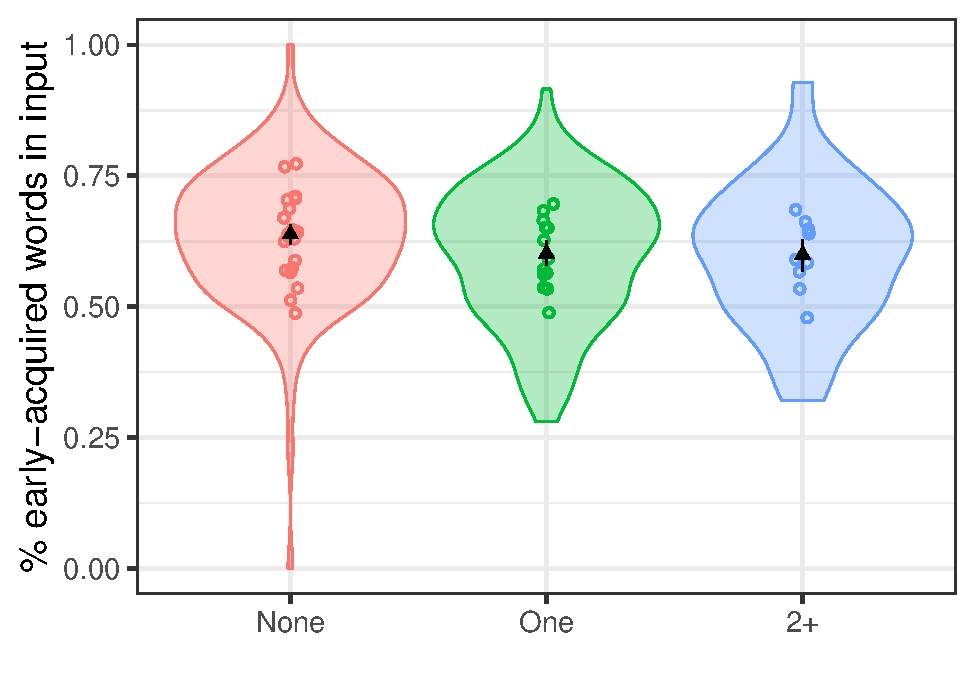
\includegraphics{SiblingsStudyText_files/figure-latex/Figure-in-cdi-1.pdf}
\caption{\label{fig:Figure-in-cdi}Proportion of early-acquired words in the input, across sibling groups. Error bars indicate mean learnable words heard across groups, with bootstrapped 95\% CIs computed over all data. Dots indicate mean number of early-acquired words per infant, collapsed across age and jittered horizontally for visual clarity.}
\end{figure}

\hypertarget{object-presence}{%
\subsubsection{Object presence}\label{object-presence}}

\begin{figure}
\centering
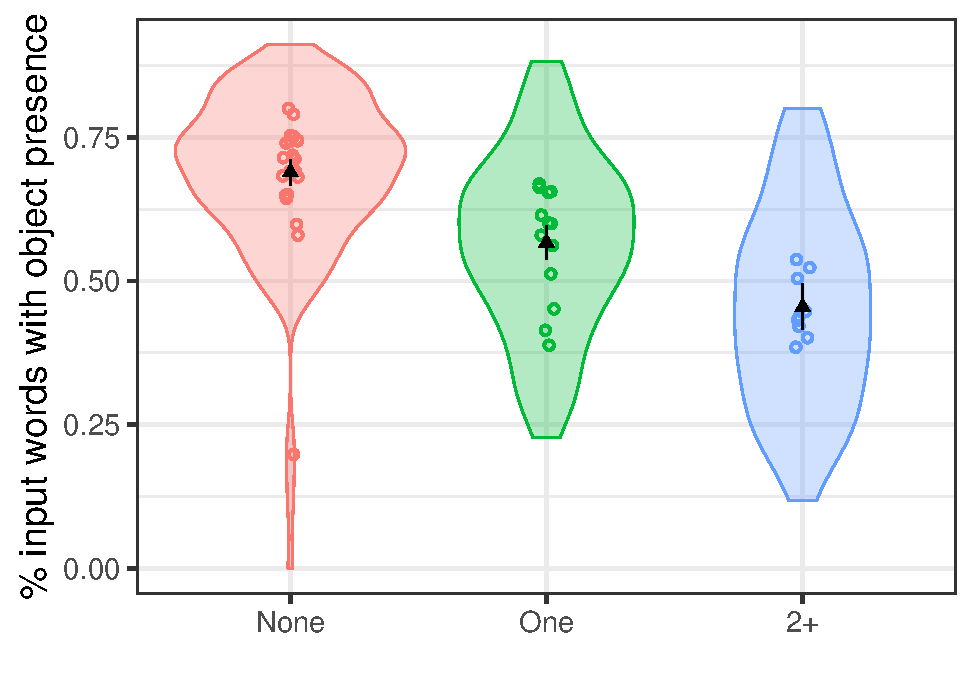
\includegraphics{SiblingsStudyText_files/figure-latex/Figure-object-presence-1.pdf}
\caption{\label{fig:Figure-object-presence}Proportion of input words produced with object presence in the input across sibling groups. Error bars and black triangles show 95\% CIs and mean proportion of object presence across sibling groups. Dots indicate mean proportion of object presence per infant, collapsing across age and jittered horizontally for visual clarity.}
\end{figure}

On average, 59\% of utterances were produced in the presence of the relevant object (Mdn=0.59, SD=0.12). We hypothesized that infants with more siblings would hear fewer words in referentially transparent conditions (i.e.~they would experience lower object presence) than those with fewer siblings. Indeed, modelling the quantity of object present tokens that infants heard, we find a significant effect for sibling group on object presence (\(\chi^2 (2)\) = 27.02, \emph{p}\textless{} .001). See Figure \ref{fig:Figure-object-presence}. Infants with no siblings experienced 23\% more object presence in their input than those with two or more siblings, and 12\% more than those with one sibling. Post-hoc comparisons revealed significant between-group differences: infants with no siblings experienced significantly more object presence than those with one sibling (\emph{W}=241, \emph{p}=\textless{} .001, Bonferroni corrections applied). Likewise, infants with one sibling experienced significantly more object presence those with two or more siblings (\emph{W}=19, \emph{p}=.007). See Table \ref{tab:table-data-summary}.

\hypertarget{discussion}{%
\section{Discussion}\label{discussion}}

We investigated the nature of infant language development in relation to number of children in the household. Previous research found a delay in lexical acquisition for later-born infants (Fenson et al., 1994; Hoff, 2006), with differences in input across birth order reported as a root cause. Our results add several new dimensions to this, by testing for differences across more vs.~fewer older siblings, and by looking at input child-centered home recordings. Infants with more siblings were reported to say fewer words by 18 months, heard fewer nouns from their parents, heard fewer early-acquired nouns, and experienced less \enquote{object presence} when hearing them.

Importantly, and in contrast with some previous research (Hoff-Ginsberg, 1998; Oshima-Takane \& Robbins, 2003), infants with one sibling showed no delay in lexical production and minimal reduction in input in comparison to first-born infants. That is, our results suggest that simply having a sibling does not contribute to input or vocabulary differences across children (as measured here), while having more than one siblings seems to do so. Indeed, infants with zero and one sibling had similar results for productive vocabulary, parental noun input overall, and early-acquired nouns in the input (but not object presence, which we return to below). In contrast, infants with two or more siblings said fewer words and had lower rates of all of our input measures compared with their peers.

When we considered the effect of sibling status -- that is, whether or not infants had any siblings, disregarding specific sibling number -- our findings showed that having siblings made no difference to infants' lexical production capacities. This contrasts with Hoff-Ginsberg (1998), who found that, by 18 months, laterborns exhibit lower language skills. However, Oshima-Takane and colleagues (1996) found no overall differences between first- and second-born children across a range of language measures taken at 21 months. Our finer-grained results suggest a greater role for \emph{sibling quantity} over first- vs.~later-born status. The more older siblings a child had, the lower their reported productive vocablary at 18 months. This adds to findings from Fenson and colleagues (1994), who found a weak but significant negative correlation between birth order and production of both words and gestures. Controlling for age, our model showed that for each additional older sibling, infants produced more than 30\% fewer words by 18 months.

While infants with more siblings heard less parental input, having one sibling did not significantly reduce an infant's noun input quantity. This is in direct contrast with reports from the literature; Hoff (2006) states that \enquote{when a sibling is present, each child receives less speech directed solely at\ldots her \emph{because mothers produce the same amount of speech whether interacting with one or two children}} (p.67, italics added). While this does not appear to be the case in the present dataset, it may be due to the circumstances of the home-recorded data. While siblings were present in many of the recordings, given the focus of the data collection, parents may have had a tendency to direct their attention - and consequently their linguistic input - more towards the target child.

Looking at input to infants with two or more siblings, the picture is strikingly different: these infants heard around 50\% fewer input words in any given session than their first- or second-born peers. The existing language development literature makes a convincing case for the importance of input quantity in regard to lexicon size in early development (Huttenlocher et al., 1991; Ramírez-Esparza et al., 2014), and we see this reflected in our results. From our sample of 44 participants, the infants who heard fewer input words over the 17 months of data collection also had smaller vocabularies by 1;6. These results add a new perspective to the literature on the \enquote{sibling effect}. As far as we are aware, no other studies have considered how amount of parental input differs in relation to more versus fewer siblings - research in this area is limited to analyses of first- versus second-born children. Furthermore, Oshima-Takane and Robbins' (2003) findings contrast with those reported here: in their study of dyadic vs.~triadic interactions between mothers and their children (infant + sibling or infant only), maternal input directed at the infant was lower in the triadic interaction. However, given that their recordings were carried out in a lab setting, their data may not represent the fully naturalistic interactions that we are more likely to expect in home-recorded data: second-born children may have received more linguistic attention in the lab, especially when under experimental conditions.

Infants' exposure to early-acquired (CDI) words was affected by sibling number; again, infants with more siblings were at a disadvantage overall, but having one sibling did not affect the number of early-acquired words heard in the input compared to zero siblings. This qualitative measure takes into account a number of factors known to be important in early word learning. One such factor is input frequency (Ambridge, Kidd, Rowland, \& Theakston, 2015): the more frequently an infant hears a word, the more likely she is to acquire that form early on. Given that 60\% of over 83,000 noun tokens in the input data matched the 241 object words on the CDI form, we can reliably assume that word repetition was high. Words acquired early in development (and thus included on the CDI form) tend to be learnable in other important ways: they may be phonologically well-suited to infants' early production capacity (e.g.~phonologically simple forms: Laing, 2019, p. @vihman\_prosodic\_2016, or forms that are pragmatically salient such as sound effects or animal sounds 2014), they may be produced frequently in isolation (e.g.~\textbf{mommy}, \textbf{baby}; Brent \& Siskind, 2001), or they may be labels for concrete items that are common in the infant's surroundings (e.g.~\textbf{bottle}, \textbf{mouth}; Bergelson \& Swingley, 2012). It is perhaps unsurprising that infants with more siblings tended to hear fewer early-acquired words in our data: a higher number of older siblings in the household almost tautologically ensures more complex grammatical structures, fewer concrete words, and more pronouns spoken to and by these children (Oshima-Takane et al., 1996).

Input disadvantages were most marked in our analysis of object presence. In this case, even having one sibling led to fewer word-object pairs presented in the input. Presence of a labelled object with congruent input speech is known to be supportive in early word learning. Gogate and colleagues (2000) highlight the importance of object presence in relation to contingent word production, which supports the learning of novel word-object combinations. They report that \enquote{multimodal motherese} - whereby a target word is produced in synchrony with its referent, often involving movement or touch of the object - supports word learning by demonstrating novel word-object combinations in their infant's input. Lower rates of referential transparency in children's input have also been proposed to explain why common non-nouns like \emph{hi} and \emph{uh-oh} are learned later than concrete nouns (Bergelson \& Swingley, 2013).

Our results indicated a relatively close link between input and early production: children with two or more siblings said the fewest words and heard the lowest quantity and quality input, as operationalized by our measures. Similarly, infants with 0 or 1 sibling showed similar production levels, parental input, and presence of early-acquired words in the input. Object presence varied more linearly across sibling quantity, suggesting it may be a less critical driver of early word production. Alternatively, the reduced object presence for children with 1 sibling may have been compensated for in other ways we did not measure here, which in turn resulted in the indistinguishable vocabulary in the 0 and 1 sibling children at 17 months.

More generally, one possibility raised by these results is that perhaps parents are able to compensate or provide relatively similar input and learning support for one or two children, but once children outnumber parents, this balancing act of attention, care, and time, becomes unwieldy. While the current sample is relatively limited and homogenous in the family structures and demographics it includes, future work could fruitfully investigate this possibility by considering whether (controlling for other potential contributors like SES, Hoff-Ginsberg, 1998) the presence of more caregivers (whether parents, relatives, or other adults) helps foster language development.

Alternatively, second-borns might \enquote{even out} with children with no siblings due to a trade-off between direct attention from the caregiver and the possibility of more sophisticated social-communicative interactions. For these infants there is still ample opportunity to engage with the mother in one-to-one interactions, allowing a higher share of her attention than is available to third- or later-borns. Furthermore, triadic interactions can benefit the development of a number of linguistic and communication skills (Barton \& Tomasello, 1991; Dunn \& Shatz, 1989). Second-borns may also benefit from overheard speech in their input, supporting the acquisition of nouns and even more complex lexical categories (Floor \& Akhtar, 2006; Oshima-Takane et al., 1996). For infants with one sibling, the benefits of observing/overhearing interactions between sibling and caregiver, as well as the possibility for partaking in such interactions, may outweigh the decrease in some aspects of the input (i.e., in our data, only observed in object presence). Having more than one sibling may throw this off-balance.

Importantly, the present results make no claims about eventual outcomes for these children: generally speaking, regardless of sibling number, all typically-developing infants generally reach full and fluent language use. Indeed, some research suggests that sibling effects, while they may be clear in early development, are not always sustained into childhood; e.g.~twins are known to experience a delay in language development into the third year, but are quick to catch up thereafter (Dales, 1969; Tomasello, Mannle, \& Kruger, 1986). This demonstrates the cognitive adaptability of early development, which brings about the acquisition of language across varying and allegedly \enquote{imperfect} learning environments. Infants' capacity to develop linguistic skills from the resources that are available to them -- whether that is infant-directed object labels or overheard abstract concepts -- highlights the dynamic and adaptable nature of early cognitive development, and a system that is sufficiently robust to bring about the same outcome across populations.

Of course, the \enquote{success} of early language development is defined by the goals that we set in this domain. Here we chose word production as our measure of linguistic capability; we did not consider other, equally valid measures such as language comprehension or early social-interaction skills. Similarly, our input measures focused on nouns; other lexical classes may reveal different effects, though they are generally sparser until toddlerhood. There is also some imbalance in group sizes across our data; our sample was not pre-selected for sibling number, and so group sizes are unmatched across the analysis. Including a larger number of infants with 2+ siblings may have revealed a different pattern of results. Finally, more work across wider and larger populations is necessary to unpack the generalizability of the present results. Our sample is refelective of average household sizes in middle-class families across North America and Western Europe (Office for National Statistics, 2018; United States Census Bureau, 2010), but it is not unusual in some communities and parts of the world for couples to have between three and six children in their household on average (Institute for Family Studies \& Wheatley Institution, 2019). Adding to this, it is also necessary to consider cross-cultural differences in the way children are addressed by their parents. In a study of the early input experienced by children growing up in a Tseltal Mayan village, Casillas, Brown and Levinson (2019) found that almost all of children's input came from speech directed at other people (21 minutes per hour, compared with just under 4 minutes/hour of specifically child-directed input). However, they did not hear much input from siblings, which contrasts with findings from Shneidman and Goldin-Meadow (2012), who found that 69\% of speech directed at Mayan children came from their siblings (in comparison with 10\% for children in the USA).

In conclusion, our results support the general findings from the literature showing a disadvantage in lexical acquisition for later-born infants in relation to their first-born peers. However, we highlight an important difference from previous findings, namely that in the present sample, second-born infants are at no disadvantage overall, while infants with more than two siblings are. We related this directly to the infants' input over a period of one year: infants' productive vocabulary was reflective of the input quality in their home environment, and both were influenced by sibling number. As reported in longitudinal studies mapping early language outcomes with later educational success (Lee, 2011; Marchman \& Fernald, 2008), the differences we observe in the early input here may have longer-term implications for children born into households with more older children. As has been noted in studies across a range of domains (e.g.~Esposito et al., 2020; Kantarevic \& Mechoulan, 2006), higher sibling number may have a detrimental effect across the lifespan. These finding point to the potential importance of the early language environment, which may be a key factor in the broader research that shows the \enquote{sibling effect} to have negative economic and social implications.

\newpage

\hypertarget{references}{%
\section{References}\label{references}}

\begingroup
\setlength{\parindent}{-0.5in}
\setlength{\leftskip}{0.5in}

\hypertarget{refs}{}
\leavevmode\hypertarget{ref-ambridge_ubiquity_2015}{}%
Ambridge, B., Kidd, E., Rowland, C. F., \& Theakston, A. L. (2015). The ubiquity of frequency effects in first language acquisition. \emph{Journal of Child Language}, \emph{42}(2), 239--273.

\leavevmode\hypertarget{ref-anderson_linking_2021}{}%
Anderson, N. J., Graham, S. A., Prime, H., Jenkins, J. M., \& Madigan, S. (2021). Linking quality and quantity of parental linguistic input to child language skills: A meta-analysis. \emph{Child Development}, \emph{92}(2), 484--501. \url{https://doi.org/10.1111/cdev.13508}

\leavevmode\hypertarget{ref-anderson_vocabulary_1981}{}%
Anderson, R. C., \& Freebody, P. (1981). Vocabulary knowledge. In \emph{In t. Guthrie (ed.), comprehension and teaching: Research reviews} (pp. 77--117). Newark, DE: International Reading Association.

\leavevmode\hypertarget{ref-barton_joint_1991}{}%
Barton, M. E., \& Tomasello, M. (1991). Joint attention and conversation in mother-infant-sibling triads, \emph{62}(3), 517--529.

\leavevmode\hypertarget{ref-behrman_birth_1986}{}%
Behrman, J. R., \& Taubman, P. (1986). Birth order, schooling, and earnings. \emph{Journal of Labor Economics}, \emph{4}(3), S121--S145. Retrieved from \url{https://www.jstor.org/stable/2534958}

\leavevmode\hypertarget{ref-bergelson_day_2019}{}%
Bergelson, E., Amatuni, A., Dailey, S., Koorathota, S., \& Tor, S. (2019). Day by day, hour by hour: Naturalistic language input to infants. \emph{Developmental Science}, \emph{22}(1), e12715. \url{https://doi.org/10.1111/desc.12715}

\leavevmode\hypertarget{ref-bergelson_nature_2017}{}%
Bergelson, E., \& Aslin, R. N. (2017). Nature and origins of the lexicon in 6-mo-olds. \emph{Proceedings of the National Academy of Sciences}, \emph{114}(49), 12916--12921. \url{https://doi.org/10.1073/pnas.1712966114}

\leavevmode\hypertarget{ref-bergelson_at_2012}{}%
Bergelson, E., \& Swingley, D. (2012). At 6-9 months, human infants know the meanings of many common nouns. \emph{Proceedings of the National Academy of Sciences}. \url{https://doi.org/10.1073/pnas.1113380109}

\leavevmode\hypertarget{ref-bergelson_acquisition_2013}{}%
Bergelson, E., \& Swingley, D. (2013). The acquisition of abstract words by young infants. \emph{Cognition}, \emph{127}(3), 391--397. \url{https://doi.org/10.1038/jid.2014.371}

\leavevmode\hypertarget{ref-berglund_communicative_2005}{}%
Berglund, E., Eriksson, M., \& Westerlund, M. (2005). Communicative skills in relation to gender, birth order, childcare and socioeconomic status in 18-month-old children. \emph{Scandinavian Journal of Psychology}, \emph{46}(6), 485--491. \url{https://doi.org/10.1111/j.1467-9450.2005.00480.x}

\leavevmode\hypertarget{ref-black_healthy_2016}{}%
Black, S. E., Devereux, P. J., \& Salvanes, K. G. (2016). Healthy(?), Wealthy, and wise: Birth order and adult health. \emph{Economics \& Human Biology}, \emph{23}, 27--45. \url{https://doi.org/10.1016/j.ehb.2016.06.005}

\leavevmode\hypertarget{ref-braginsky_consistency_2019}{}%
Braginsky, M., Yurovsky, D., Marchman, V. A., \& Frank, M. C. (2019). Consistency and variability in children's word learning across languages. \emph{Open Mind}, \emph{3}, 52--67. \url{https://doi.org/10.1162/opmi_a_00026}

\leavevmode\hypertarget{ref-brent_role_2001}{}%
Brent, M. R., \& Siskind, J. M. (2001). The role of exposure to isolated words in early vocabulary development. \emph{Cognition}, \emph{81}(2), 33--44. \url{https://doi.org/10.1016/S0010-0277(01)00122-6}

\leavevmode\hypertarget{ref-bulgarelli_look_2020}{}%
Bulgarelli, F., \& Bergelson, E. (2020). Look who's talking: A comparison of automated and human-generated speaker tags in naturalistic day-long recordings. \emph{Behavior Research Methods}, \emph{52}(2), 641--653. \url{https://doi.org/10.3758/s13428-019-01265-7}

\leavevmode\hypertarget{ref-cartmill_quality_2013}{}%
Cartmill, E. a, Armstrong, B. F., Gleitman, L. R., Goldin-Meadow, S., Medina, T. N., \& Trueswell, J. C. (2013). Quality of early parent input predicts child vocabulary 3 years later. \emph{Proceedings of the National Academy of Sciences of the United States of America}. \url{https://doi.org/10.1073/pnas.1309518110}

\leavevmode\hypertarget{ref-casillas_early_2019}{}%
Casillas, M., Brown, P., \& Levinson, S. C. (2019). Early language experience in a tseltal mayan village. \emph{Child Development}, \emph{EarlyView article}. \url{https://doi.org/10.1111/cdev.13349}

\leavevmode\hypertarget{ref-dales_motor_1969}{}%
Dales, R. J. (1969). Motor and language development of twins during the first three years. \emph{The Journal of Genetic Psychology; Provincetown, Mass., Etc.}, \emph{114}(2), 263--271. Retrieved from \url{https://search.proquest.com/docview/1297124434/citation/D928716F9A7E4AEFPQ/1}

\leavevmode\hypertarget{ref-dunn_becoming_1989}{}%
Dunn, J., \& Shatz, M. (1989). Becoming a conversationalist despite (or because of) having an older sibling. \emph{Child Development}, \emph{60}(2), 399--410.

\leavevmode\hypertarget{ref-esposito_importance_2020}{}%
Esposito, L., Kumar, S. M., \& Villaseñor, A. (2020). The importance of being earliest: Birth order and educational outcomes along the socioeconomic ladder in mexico. \emph{Journal of Population Economics}. \url{https://doi.org/10.1007/s00148-019-00764-3}

\leavevmode\hypertarget{ref-fenson_variability_1994}{}%
Fenson, L., Dale, P. S., Reznick, J. S., Bates, E., Thal, D. J., Pethick, M., Stephen J. Tomasello, \ldots{} Stiles, J. (1994). Variability in early communicative development. \emph{Monographs of the Society for Research in Child Development}, \emph{59}. \url{https://doi.org/10.2307/1166093}

\leavevmode\hypertarget{ref-fenson_macarthur-bates_2007}{}%
Fenson, L., Marchman, V. A., Thal, D. J., Dale, P. S., Reznick, J. S., \& Bates, E. (2007). \emph{MacArthur-bates communicative development inventories} (2nd ed.). Baltimore, MD: Paul H. Brookes Publishing Co.

\leavevmode\hypertarget{ref-ferjan_ramirez_parent_2020}{}%
Ferjan Ramírez, N., Lytle, S. R., \& Kuhl, P. K. (2020). Parent coaching increases conversational turns and advances infant language development. \emph{Proceedings of the National Academy of Sciences}, 201921653. \url{https://doi.org/10.1073/pnas.1921653117}

\leavevmode\hypertarget{ref-floor_can_2006}{}%
Floor, P., \& Akhtar, N. (2006). Can 18-month-old infants learn words by listening in on conversations? \emph{Infancy}, \emph{9}(3), 327--339. \url{https://doi.org/10.1207/s15327078in0903_4}

\leavevmode\hypertarget{ref-frank_variability_2021}{}%
Frank, M. C., Braginsky, M., Yurovsky, D., \& Marchman, V. A. (2021). \emph{Variability and consistency in early language learning: The wordbank project}. MIT Press.

\leavevmode\hypertarget{ref-galton_english_1874}{}%
Galton, F. (1874). \emph{English men of science: Their nature and nurture}. London: MacMillan.

\leavevmode\hypertarget{ref-gleitman_hard_2005}{}%
Gleitman, L. R., Cassidy, K., Nappa, R., Papafragou, A., \& Trueswell, J. C. (2005). Hard words. \emph{Language Learning and Development}, \emph{1}(1), 23--64. \url{https://doi.org/10.1207/s15473341lld0101_4}

\leavevmode\hypertarget{ref-gogate_study_2000}{}%
Gogate, L. J., Bahrick, L. E., \& Watson, J. D. (2000). A study of multimodal motherese: The role of temporal synchrony between verbal labels and gestures. \emph{Child Development}, \emph{71}(4), 878--894. \url{https://doi.org/10.1111/1467-8624.00197}

\leavevmode\hypertarget{ref-havron_effect_2019}{}%
Havron, N., Ramus, F., Heude, B., Forhan, A., Cristia, A., Peyre, H., \ldots{} Thiebaugeorges, O. (2019). The effect of older siblings on language development as a function of age difference and sex. \emph{Psychological Science}, \emph{30}(9), 1333--1343. \url{https://doi.org/10.1177/0956797619861436}

\leavevmode\hypertarget{ref-hoff_how_2006}{}%
Hoff, E. (2006). How social contexts support and shape language development. \emph{Developmental Review}, \emph{26}(1), 55--88. \url{https://doi.org/10.1016/j.dr.2005.11.002}

\leavevmode\hypertarget{ref-hoff-ginsberg_mother-child_1991}{}%
Hoff-Ginsberg, E. (1991). Mother-child conversation in different social classes and communicative settings. \emph{Child Development}, \emph{62}(4), 782--796. \url{https://doi.org/10.2307/1131177}

\leavevmode\hypertarget{ref-hoff-ginsberg_relation_1998}{}%
Hoff-Ginsberg, E. (1998). The relation of birth order and socioeconomic status to children's language experience and language development. \emph{Applied Psycholinguistics}, \emph{19}(4), 603--629. \url{https://doi.org/10.1017/S0142716400010389}

\leavevmode\hypertarget{ref-hoff-ginsberg_older_1991}{}%
Hoff-Ginsberg, E., \& Krueger, W. M. (1991). Older siblings as conversational partners, \emph{37}(3), 465--481.

\leavevmode\hypertarget{ref-huttenlocher_early_1991}{}%
Huttenlocher, J., Haight, W., Bryk, A., Seltzer, M., \& Lyons, T. (1991). Early vocabcabulary growth: Relation to language input and gender. \emph{Developmental Psychology}, \emph{27}(2), 236--248.

\leavevmode\hypertarget{ref-institute_for_family_studies_world_2019}{}%
Institute for Family Studies, \& Wheatley Institution. (2019). \emph{World family map 2019: Mapping family change and child well-being outcomes}. Charlottesville, VA: Institute for Family Studies. Retrieved from \url{https://ifstudies.org/reports/world-family-map/2019/executive-summary}

\leavevmode\hypertarget{ref-jones_language_1987}{}%
Jones, C. P., \& Adamson, L. B. (1987). Language use in mother-child and mother-child-sibling interactions, \emph{58}(2), 356--366.

\leavevmode\hypertarget{ref-kantarevic_birth_2006}{}%
Kantarevic, J., \& Mechoulan, S. (2006). Birth order, educational attainment, and earnings: An investigation using the PSID. \emph{Journal of Human Resources}, \emph{XLI}(4), 755--777. \url{https://doi.org/10.3368/jhr.XLI.4.755}

\leavevmode\hypertarget{ref-kuznetsova_lmertest_2017}{}%
Kuznetsova, A., Brockhoff, P. B., \& Christensen, R. H. B. (2017). \{lmerTest\} package: Tests in linear mixed effects models. \emph{Journal of Statistical Software}, \emph{82}(13), 1--26. \url{https://doi.org/10.18637/jss.v082.i13}

\leavevmode\hypertarget{ref-laing_role_2019}{}%
Laing, C. (2019). A role for onomatopoeia in early language: Evidence from phonological development. \emph{Language and Cognition}, \emph{11}(2), 173--187. \url{https://doi.org/10.1017/langcog.2018.23}

\leavevmode\hypertarget{ref-laing_phonological_2014}{}%
Laing, C. E. (2014). A phonological analysis of onomatopoeia in early word production. \emph{First Language}, \emph{34}(5), 387--405. \url{https://doi.org/10.1177/0142723714550110}

\leavevmode\hypertarget{ref-lee_size_2011}{}%
Lee, J. (2011). Size matters: Early vocabulary as a predictor of language and literacy competence. \emph{Applied Psycholinguistics}, \emph{32}(1), 69--92. \url{https://doi.org/10.1017/S0142716410000299}

\leavevmode\hypertarget{ref-marchman_speed_2008}{}%
Marchman, V. A., \& Fernald, A. (2008). Speed of word recognition and vocabulary knowledge in infancy predict cognitive and language outcomes in later childhood. \emph{Developmental Science}, \emph{11}(3), F9--F16. \url{https://doi.org/10.1111/j.1467-7687.2008.00671.x}

\leavevmode\hypertarget{ref-mcgillion_randomised_2017}{}%
McGillion, M., Pine, J. M., Herbert, J. S., \& Matthews, D. (2017). A randomised controlled trial to test the effect of promoting caregiver contingent talk on language development in infants from diverse socioeconomic status backgrounds. \emph{Journal of Child Psychology and Psychiatry}, \emph{58}(10), 1122--1131. \url{https://doi.org/10.1111/jcpp.12725}

\leavevmode\hypertarget{ref-monfardini_birth_2016}{}%
Monfardini, C., \& See, S. G. (2016). Birth order and child cognitive outcomes: An exploration of the parental time mechanism. \emph{Education Economics}, \emph{24}(5), 481--495. \url{https://doi.org/10.1080/09645292.2015.1117581}

\leavevmode\hypertarget{ref-moore_point_2019}{}%
Moore, C., Dailey, S., Garrison, H., Amatuni, A., \& Bergelson, E. (2019). Point, walk, talk: Links between three early milestones, from observation and parental report. \emph{Developmental Psychology}. \url{https://doi.org/10.1037/dev0000738}

\leavevmode\hypertarget{ref-office_for_national_statistics_families_2018}{}%
Office for National Statistics. (2018). \emph{Families with dependent children by number of children, UK, 1996 to 2017} (No. 008855). Office for National Statistics. Retrieved from \url{https://www.ons.gov.uk/peoplepopulationandcommunity/birthsdeathsandmarriages/families/adhocs/008855familieswithdependentchildrenbynumberofchildrenuk1996to2017}

\leavevmode\hypertarget{ref-oshima-takane_birth_1996}{}%
Oshima-Takane, Y., Goodz, E., \& Derevensky, J. L. (1996). Birth order effects on early language development : Do secondborn children learn from overheard speech ? Author ( s ): Yuriko oshima-takane , elizabeth goodz and jeffrey l . Derevensky published by : Wiley on behalf of the society for research in child de, \emph{67}(2), 621--634.

\leavevmode\hypertarget{ref-oshima-takane_linguistic_2003}{}%
Oshima-Takane, Y., \& Robbins, M. (2003). Linguistic environment of secondborn children. \emph{First Language}, \emph{23}(1), 21--40. \url{https://doi.org/http://dx.doi.org/10.1177/0142723703023001002}

\leavevmode\hypertarget{ref-pine_variation_1995}{}%
Pine, J. M. (1995). Variation in vocabulary development as a function of birth order. \emph{Child Development}, \emph{66}(1), 272--281.

\leavevmode\hypertarget{ref-ramirez-esparza_look_2014}{}%
Ramírez-Esparza, N., García-Sierra, A., \& Kuhl, P. K. (2014). Look who's talking: Speech style and social context in language input to infants are linked to concurrent and future speech development. \emph{Developmental Science}, \emph{17}(6), 880--891. \url{https://doi.org/10.1016/j.surg.2006.10.010.Use}

\leavevmode\hypertarget{ref-r_core_team_r_2019}{}%
R Core Team. (2019). \emph{R: A language environment for statistical computing}. R Foundation for Statistical Computing. Retrieved from \url{https://www.R-project.org/}

\leavevmode\hypertarget{ref-shneidman_language_2012}{}%
Shneidman, L. A., \& Goldin‐Meadow, S. (2012). Language input and acquisition in a mayan village: How important is directed speech? \emph{Developmental Science}, \emph{15}(5), 659--673. \url{https://doi.org/10.1111/j.1467-7687.2012.01168.x}

\leavevmode\hypertarget{ref-soderstrom_beyond_2007}{}%
Soderstrom, M. (2007). Beyond babytalk: Re-evaluating the nature and content of speech input to preverbal infants. \emph{Developmental Review}, \emph{27}(4), 501--532. \url{https://doi.org/10.1016/j.dr.2007.06.002}

\leavevmode\hypertarget{ref-stafford_maternal_1987}{}%
Stafford, L. (1987). Maternal input to twin and singleton children implications for language acquisition. \emph{Human Communication Research}, \emph{13}(4), 429--462. \url{https://doi.org/10.1111/j.1468-2958.1987.tb00114.x}

\leavevmode\hypertarget{ref-stern_prosody_1983}{}%
Stern, D. N., Spieker, S., Barnett, R. K., \& MacKain, K. (1983). The prosody of maternal speech: Infant age and context related changes. \emph{Journal of Child Language}, \emph{10}(1), 1--15. \url{https://doi.org/10.1017/S0305000900005092}

\leavevmode\hypertarget{ref-tomasello_linguistic_1986}{}%
Tomasello, M., Mannle, S., \& Kruger, A. C. (1986). Linguistic environment of 1- to 2-year-old twins. \emph{Developmental Psychology}, \emph{22}(2), 169--176. \url{https://doi.org/10.1037/0012-1649.22.2.169}

\leavevmode\hypertarget{ref-united_states_census_bureau_household_2010}{}%
United States Census Bureau. (2010). \emph{Household type by number of people under 18 years} (No. PCT16). Retrieved from \url{https://data.census.gov/cedsci/table?q=number\%20of\%20children\&hidePreview=false\&tid=DECENNIALSF12010.PCT16\&t=Children\&vintage=2018}

\leavevmode\hypertarget{ref-vihman_prosodic_2016}{}%
Vihman, M. (2016). Prosodic structures and templates in bilingual phonological development. \emph{Bilingualism: Language and Cognition}, \emph{19}(1), 69--88. \url{https://doi.org/10.1017/S1366728914000790}

\leavevmode\hypertarget{ref-wellen_effects_1985}{}%
Wellen, C. J. (1985). Effects of older siblings on the language young children hear and produce. \emph{Journal of Speech and Hearing Disorders}, \emph{50}(1), 84--99. \url{https://doi.org/10.1044/jshd.5001.84}

\leavevmode\hypertarget{ref-woollett_influence_1986}{}%
Woollett, A. (1986). The influence of older siblings on the language environment of young children. \emph{British Journal of Developmental Psychology}, \emph{4}, 235--245.

\leavevmode\hypertarget{ref-yurovsky_statistical_2013}{}%
Yurovsky, D., Smith, L. B., \& Yu, C. (2013). Statistical word learning at scale: The baby's view is better. \emph{Developmental Science}, \emph{16}(6), 959--966. \url{https://doi.org/10.1111/desc.12036}

\leavevmode\hypertarget{ref-zambrana_impact_2012}{}%
Zambrana, I. M., Ystrom, E., \& Pons, F. (2012). Impact of gender, maternal education, and birth order on the development of language comprehension: A longitudinal study from 18 to 36 months of age. \emph{Journal of Developmental \& Behavioral Pediatrics}, \emph{33}(2), 146--155. \url{https://doi.org/10.1097/DBP.0b013e31823d4f83}

\endgroup


\end{document}
